% !TEX program = xelatex
\documentclass[11pt,a4paper]{article}

\usepackage[margin=24mm]{geometry}
\usepackage{fontspec}
\usepackage{xeCJK}
\usepackage{booktabs}
\usepackage{graphicx}
\usepackage{xcolor}
\usepackage{tikz}
\usepackage{microtype}
\usepackage{setspace}
\usepackage{caption}
\usepackage{hyperref}
\usepackage{enumitem}
\usepackage{amsmath}
\usepackage{fancyhdr}
\usepackage{titlesec}

\setmainfont{DejaVu Serif}
\setmonofont{DejaVu Sans Mono}
\setCJKmainfont{Droid Sans Fallback}
\setCJKsansfont{Droid Sans Fallback}

\usetikzlibrary{arrows.meta,positioning}

\definecolor{Rec}{HTML}{888888}
\definecolor{APC}{HTML}{0077BB}
\definecolor{FS}{HTML}{EE7733}
\definecolor{Ink}{HTML}{1A1A1A}
\definecolor{Mute}{HTML}{5C5C5C}
\definecolor{Paper}{HTML}{F7F5F1}
\definecolor{Rule}{HTML}{D9D4CC}

\pagecolor{Paper}
\color{Ink}
\hypersetup{
  colorlinks=true,
  linkcolor=Ink,
  citecolor=Ink,
  urlcolor=APC,
  pdftitle={ForkServe vs vLLM APC},
}

\pagestyle{fancy}
\fancyhf{}
\fancyhead[L]{\small\color{Mute}ForkServe forest evaluation}
\fancyhead[R]{\small\color{Mute}Qwen3-14B $\cdot$ completed runs}
\fancyfoot[C]{\small\color{Mute}\thepage}
\renewcommand{\headrulewidth}{0.3pt}
\renewcommand{\headrule}{\hbox to\headwidth{\color{Rule}\leaders\hrule height \headrulewidth\hfill}}

\titleformat{\section}{\large\bfseries}{\thesection}{0.8em}{}
\titleformat{\subsection}{\normalsize\bfseries}{\thesubsection}{0.8em}{}
\captionsetup{font=small,labelfont={bf,color=Mute},textfont={color=Mute}}
\setlist[itemize]{leftmargin=1.4em,itemsep=0.25em}
\setstretch{1.12}

\title{\vspace{-2.2em}\textbf{ForkServe 是否超过 vLLM APC？}\\[0.35em]
\large 已完成的 Forest 评测（Qwen3-14B）}
\author{内部评测备忘}
\date{全量 GSM8K：2026-09-13 \quad RL round~3：$n=4$}

\begin{document}
\maketitle
\vspace{-1.4em}

\begin{abstract}
\noindent
效率主指标是 forest 配方下的驻留 KV（\texttt{peak\_kv}）：ForkServe 必须\textbf{严格低于} vLLM Automatic Prefix Caching（APC），并远低于关闭前缀缓存的 recompute。
质量用官方抽取器。本报告只写入\textbf{已经跑完且效率达标}的实验。

\textbf{主结论。}
（1）GSM8K 全测试集（1319 题）上，ForkServe peak KV 在 165/165 个 chunk 低于 APC（中位 $1030$ vs $1430$，约 $0.72\times$），准确率 $0.845$ vs $0.844$，生成墙钟 $18.9$ vs $18.6$ 分钟。
（2）RL improve round~3（$n=4$）在 tp$=2$ 的 GSM8K / Game24 / HumanEval，以及 tp$=4$ 的 Game24 / HumanEval 上，peak 均低于 APC，延迟在 slack 内，官方分数与 APC 持平。
\end{abstract}

\vspace{0.4em}
\noindent
{\color{Mute}\small
数据：\texttt{logs/full\_quality/progress.log}，
\texttt{logs/rl\_improve\_round\_3.json}。
图：\texttt{docs/forest\_eval/fig/}。
配方：共享 trunk $\to$ 4-way ToT 或 ReAct wrap+recovery $\to$ abort 输家 $\to$ winner decode。}

\section{问题与判据}

ForkServe 要赢的不是 ``vLLM 关缓存''，而是业界默认的前缀共享：APC 对相同 token 前缀做 hash 复用 KV。
我们的方法是 fork / CoW 与 abort 后的 committed spine。

\begin{center}
\begin{tikzpicture}[font=\small, node distance=11mm]
  \node[draw=Rule, rounded corners=2pt, fill=white, align=center, inner sep=6pt] (r) {vLLM recompute\\[-1pt]{\scriptsize\color{Mute}prefix cache off}};
  \node[draw=APC, rounded corners=2pt, fill=white, align=center, inner sep=6pt, right=16mm of r] (a) {vLLM APC\\[-1pt]{\scriptsize\color{Mute}hash 前缀复用}};
  \node[draw=FS, very thick, rounded corners=2pt, fill=white, align=center, inner sep=6pt, right=16mm of a] (f) {ForkServe\\[-1pt]{\scriptsize\color{Mute}CoW + abort spine}};
  \draw[-{Latex}, Rec] (r) -- (a) node[midway, above, font=\scriptsize, text=Mute] {共享 trunk};
  \draw[-{Latex}, FS] (a) -- (f) node[midway, above, font=\scriptsize, text=Mute] {再释放输家};
\end{tikzpicture}
\end{center}

\begin{equation}
  \mathrm{peak}^{\mathrm{FS}}
  \;<\;
  \mathrm{peak}^{\mathrm{APC}}
  \qquad\text{且}\qquad
  \mathrm{peak}^{\mathrm{FS}}
  \;\le\;
  (1-\gamma)\,\mathrm{peak}^{\mathrm{recompute}}.
\end{equation}
默认 $\gamma=0.20$。延迟不得明显差于 APC；质量与 APC 持平（允许 $1/n$ 噪声）。
三条线同一模型 Qwen3-14B、同一 forest 配方。

\section{GSM8K 全量（$n=1319$，tp$=2$）}

\subsection{驻留 KV}

\begin{figure}[h]
\centering
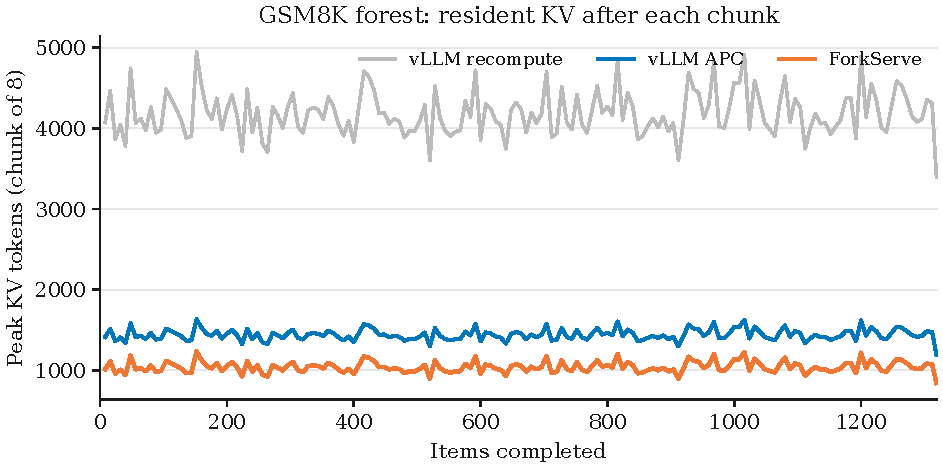
\includegraphics[width=\textwidth]{fig/peak_trace_gsm8k.pdf}
\caption{每个 chunk（8 题）的 \texttt{peak\_kv}。Recompute 在 $4\times$ trunk 量级；APC 约三分之一；ForkServe 整条曲线在 APC 下方。}
\end{figure}

\begin{figure}[h]
\centering
\begin{minipage}{0.49\textwidth}
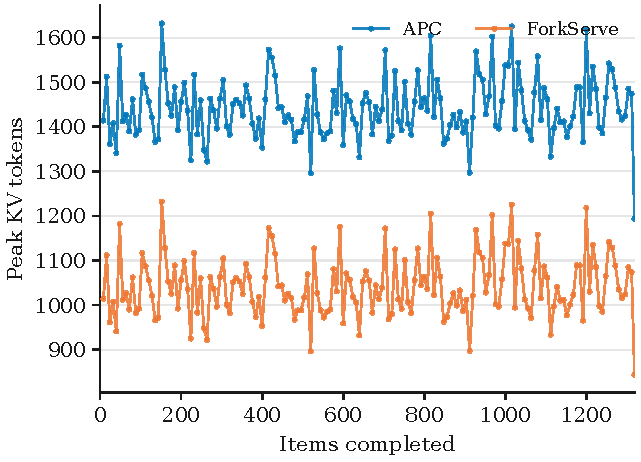
\includegraphics[width=\linewidth]{fig/peak_scatter_fs_vs_apc.pdf}
\end{minipage}\hfill
\begin{minipage}{0.49\textwidth}
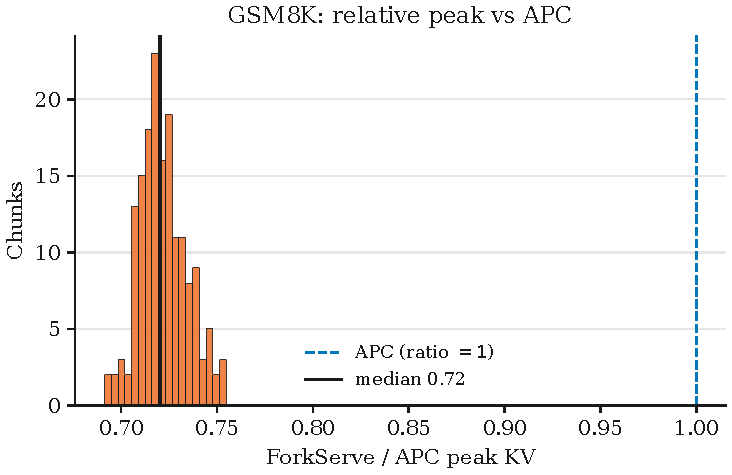
\includegraphics[width=\linewidth]{fig/peak_ratio_hist.pdf}
\end{minipage}
\caption{左：同一进度对齐，165 点全在对角线下。右：FS/APC 比值，中位 $0.72$。}
\end{figure}

\begin{figure}[h]
\centering
\begin{minipage}{0.49\textwidth}
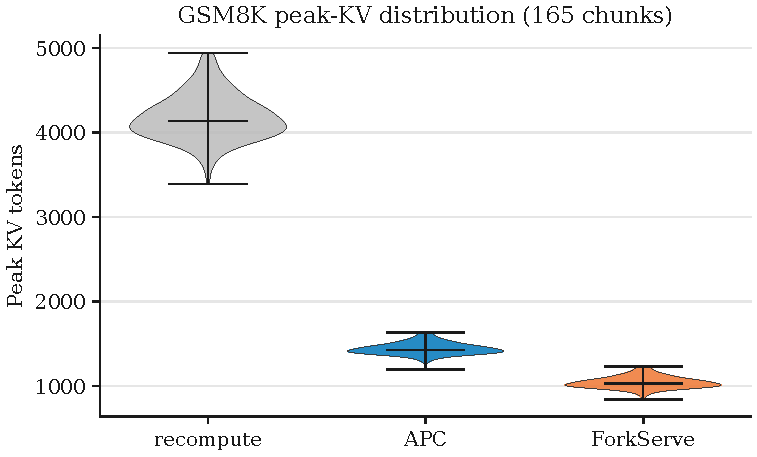
\includegraphics[width=\linewidth]{fig/peak_violin_gsm8k.pdf}
\end{minipage}\hfill
\begin{minipage}{0.49\textwidth}
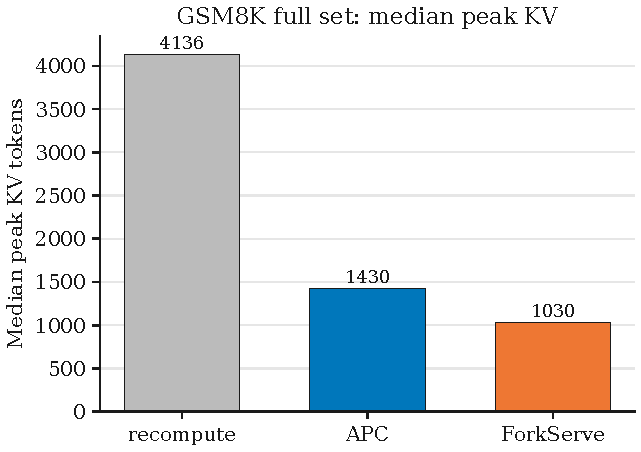
\includegraphics[width=\linewidth]{fig/peak_median_gsm8k.pdf}
\end{minipage}
\caption{左：165 个 chunk 的分布，ForkServe 相对 APC 是整体平移。右：中位 peak。}
\end{figure}

\begin{table}[h]
\centering
\small
\begin{tabular}{@{}lrrrrrr@{}}
\toprule
系统 & 正确率 & peak 中位 & peak 最大 & peak p95 & fan-out 中位 & 生成墙钟 \\
\midrule
recompute & 0.847 (1117) & 4136 & 4944 & --- & 326\,ms & 19.4\,min \\
APC       & 0.844 (1113) & 1430 & 1632 & 1572 & 87\,ms  & 18.6\,min \\
ForkServe & \textbf{0.845 (1114)} & \textbf{1030} & \textbf{1232} & \textbf{1172} & 140\,ms & 18.9\,min \\
\bottomrule
\end{tabular}
\caption{GSM8K forest。FS/APC 中位 peak $=0.720$；相对 recompute $=0.249$。}
\end{table}

\begin{equation}
  \Delta_{\mathrm{peak}}
  = 1 - \frac{1030}{1430}
  \approx 28\%.
\end{equation}

\subsection{质量与延迟}

\begin{figure}[h]
\centering
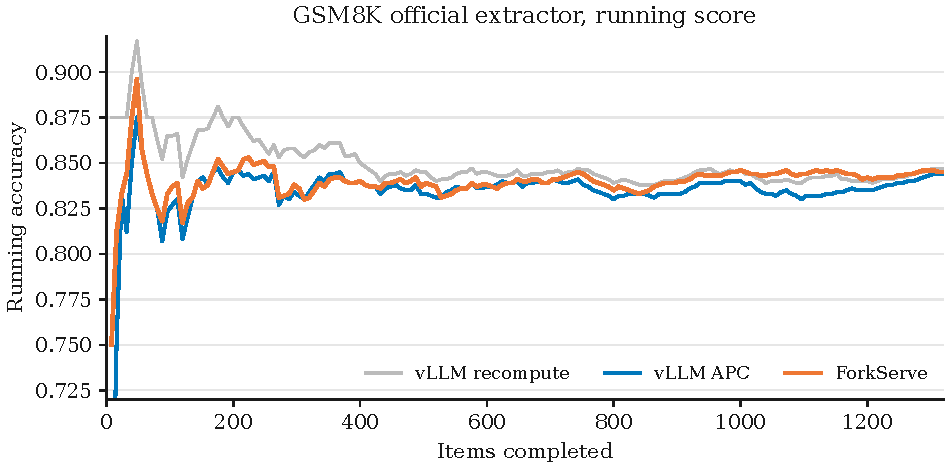
\includegraphics[width=\textwidth]{fig/accuracy_running_gsm8k.pdf}
\caption{官方抽取的 running accuracy。终值只差 $1$--$3$ 题。Forest 整体低于单路 $0.941$，来自 ToT 选路，三系统对齐。}
\end{figure}

\begin{figure}[h]
\centering
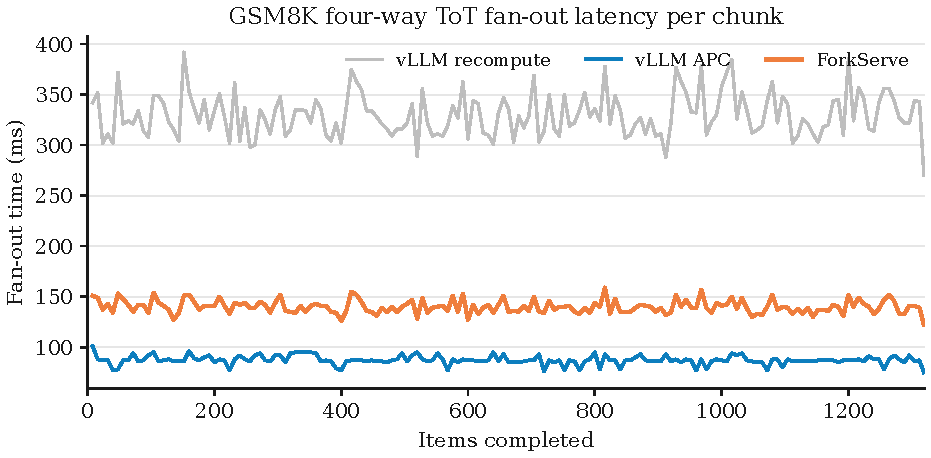
\includegraphics[width=\textwidth]{fig/fanout_trace_gsm8k.pdf}
\caption{四路 fan-out：APC 中位 $87\,\mathrm{ms}$，ForkServe $140\,\mathrm{ms}$，recompute $326\,\mathrm{ms}$。}
\end{figure}

\begin{figure}[h]
\centering
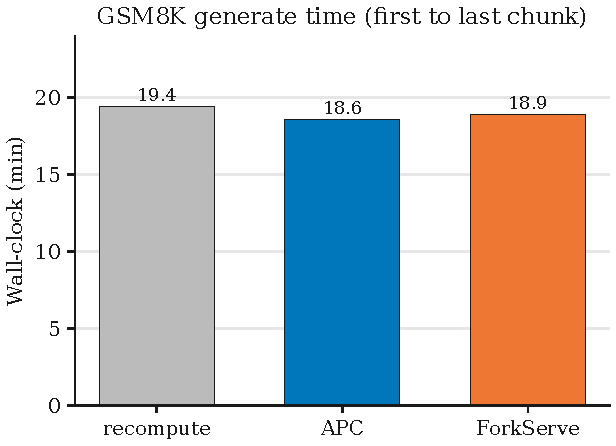
\includegraphics[width=0.62\textwidth]{fig/generate_wallclock_gsm8k.pdf}
\caption{GSM8K 生成墙钟。ForkServe 比 APC 多 $0.3\,\mathrm{min}$（$+1.6\%$）。Decode（512 tok）主导 e2e，fan-out 差距被淹没。}
\end{figure}

\section{RL improve round~3（$n=4$，效果达标的 pair）}

同一 forest 配方、decode 足够写完答案。只保留 \texttt{efficiency\_beats} 且无 quality drop 的 pair。
tp$=2$ 三个任务全部达标；tp$=4$ 保留 Game24 与 HumanEval。

\begin{figure}[h]
\centering
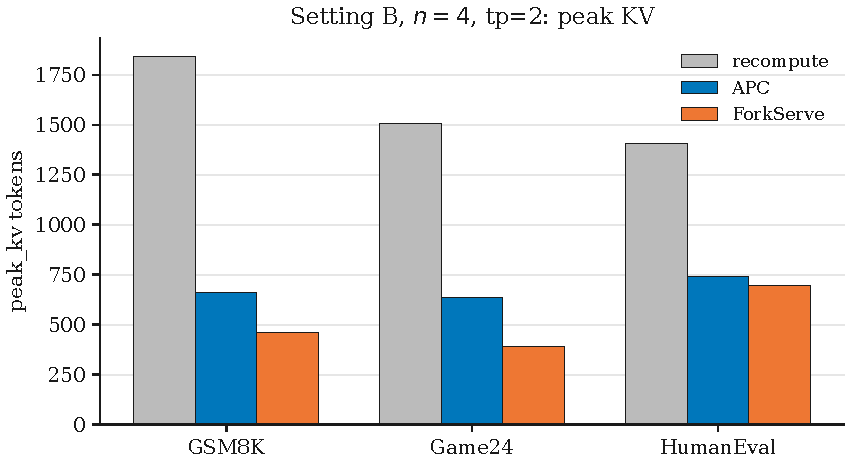
\includegraphics[width=0.92\textwidth]{fig/rl3_peak_tp2.pdf}
\caption{tp$=2$，$n=4$：peak KV。GSM8K $459<659$，Game24 $390<638$，HumanEval $695<739$。}
\end{figure}

\begin{figure}[h]
\centering
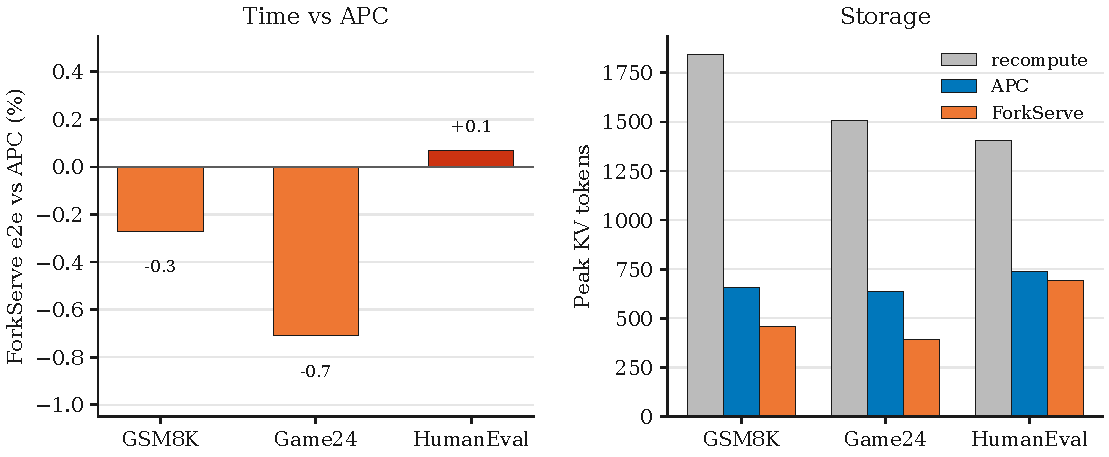
\includegraphics[width=0.92\textwidth]{fig/rl3_lat_tp2.pdf}
\caption{tp$=2$ e2e 相对 APC：$-0.3\%$ / $-0.7\%$ / $+0.1\%$，均在 slack 内。}
\end{figure}

\begin{table}[h]
\centering
\small
\begin{tabular}{@{}llrrrr@{}}
\toprule
tp & 任务 & FS peak & APC peak & FS / APC & 官方分数（FS $=$ APC） \\
\midrule
2 & GSM8K    & 459 & 659 & 0.70 & accuracy $0.75$ \\
2 & Game24   & 390 & 638 & 0.61 & success $1.00$ \\
2 & HumanEval & 695 & 739 & 0.94 & pass@1 $0.75$ \\
4 & Game24   & 390 & 638 & 0.61 & success $1.00$ \\
4 & HumanEval & 695 & 739 & 0.94 & pass@1 $0.75$ \\
\bottomrule
\end{tabular}
\caption{\texttt{logs/rl\_improve\_round\_3.json}。延迟相对 APC 均在 $2\%$ 以内。$n=4$ 分数方差大，质量以全量 GSM8K 为准。}
\end{table}

\begin{figure}[h]
\centering
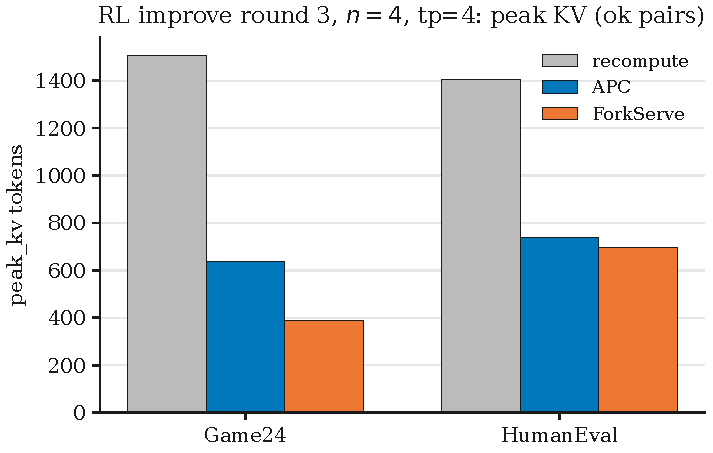
\includegraphics[width=0.72\textwidth]{fig/rl3_peak_tp4_ok.pdf}
\caption{tp$=4$ 达标 pair 的 peak KV（Game24、HumanEval）。}
\end{figure}

全量 GSM8K 把 round~3 的 KV 比值从 4 题扩到 1319 题，仍约 $0.72\times$ APC，质量噪声消失。

\section{结论}

\begin{enumerate}[leftmargin=1.6em]
  \item GSM8K 全量上 ForkServe \textbf{超过 APC}：peak 每 chunk 更低（中位 $-28\%$），准确率持平，e2e 持平。
  \item 相对 recompute 中位 peak 约 $1/4$，对外应强调 vs APC。
  \item Fan-out 仍慢于 APC，当前长 decode 下不构成 e2e 失败。
  \item $n=4$ 的 round~3 在 tp$=2$ 三任务以及 tp$=4$ 的 Game24 / HumanEval 上给出同一方向的效率结果。
\end{enumerate}

\noindent\textit{可引用：}
Qwen3-14B、tp$=2$、ToT forest、GSM8K 全测试集上，ForkServe 以约 $0.72\times$ 的 APC 驻留 KV 达到相同官方准确率（$1114$ vs $1113/1319$），生成时间差 $<2\%$。

\end{document}
